% Vertical (portrait) tree-search figure for the A0 poster.
% Same loop as REPORT_v6 Figure 2, re-proportioned top-to-bottom:
% the exit box moves to the BOTTOM of the spine so the whole column
% reads strictly downward and terminates at the deliverable.
\documentclass[tikz,border=2mm]{standalone}
\usetikzlibrary{positioning,arrows.meta,calc}
\definecolor{flowblue}{HTML}{DAE8FC}\definecolor{flowblueline}{HTML}{6C8EBF}
\definecolor{flowgreen}{HTML}{D5E8D4}\definecolor{flowgreenline}{HTML}{82B366}
\definecolor{flowpurple}{HTML}{E1D5E7}\definecolor{flowpurpleline}{HTML}{9673A6}
\definecolor{flowgrey}{HTML}{F5F5F5}\definecolor{flowgreyline}{HTML}{999999}
\begin{document}
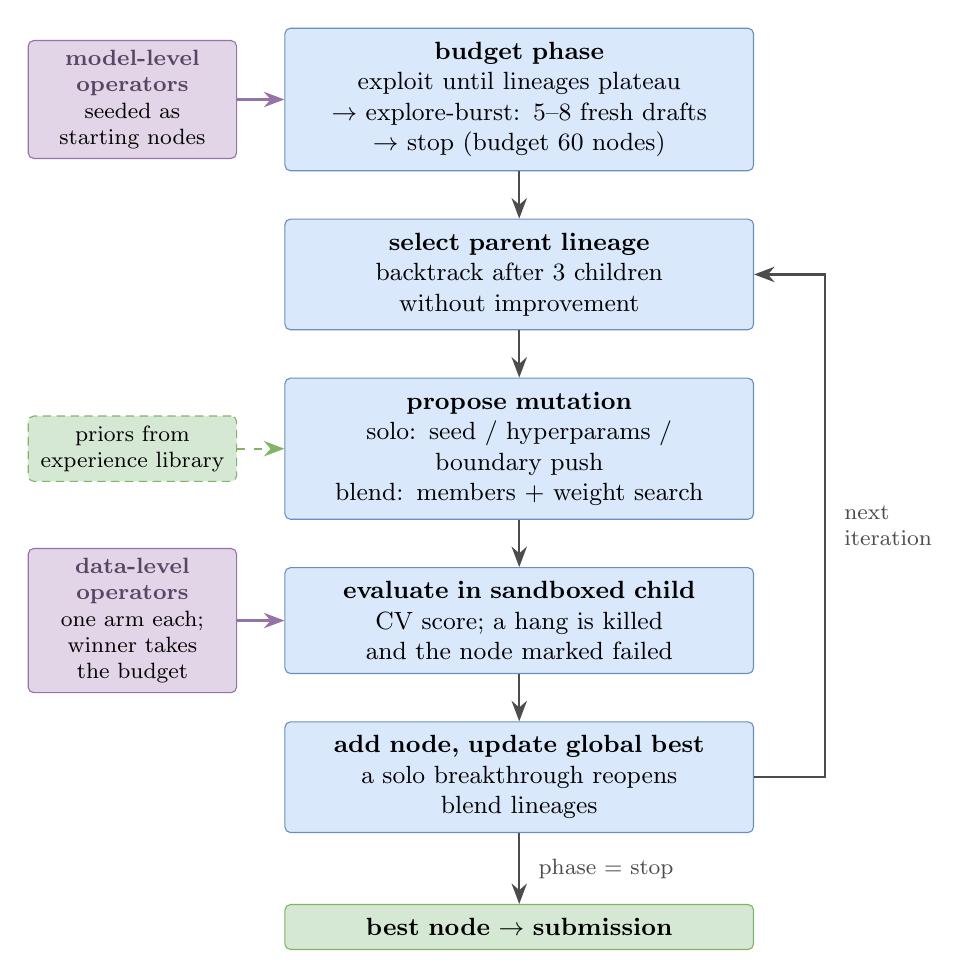
\begin{tikzpicture}[
  font=\small,
  sbox/.style={draw=flowblueline, rounded corners=2pt, align=center, inner sep=5pt,
               fill=flowblue, text width=56mm},
  sidebox/.style={draw=flowgreyline, rounded corners=2pt, align=center, inner sep=3.5pt,
                  fill=flowgrey, text width=24mm, font=\footnotesize},
  injside/.style={sidebox, fill=flowpurple, draw=flowpurpleline},
  arr/.style={-{Stealth[length=2.6mm]}, thick, black!70},
  parr/.style={-{Stealth[length=2.6mm]}, thick, flowpurpleline},
  barr/.style={parr},
  darr/.style={arr, dashed},
  lab/.style={font=\footnotesize, inner sep=1.5pt},
  node distance=6mm
]
% ----- main loop spine (top -> bottom) -----
\node[sbox] (phase) {\textbf{budget phase}\\exploit until lineages plateau\\$\to$ explore-burst: 5--8 fresh drafts\\$\to$ stop (budget 60 nodes)};
\node[sbox, below=of phase] (select) {\textbf{select parent lineage}\\backtrack after 3 children\\without improvement};
\node[sbox, below=of select] (propose) {\textbf{propose mutation}\\solo: seed / hyperparams /\\boundary push\\blend: members + weight search};
\node[sbox, below=of propose] (eval) {\textbf{evaluate in sandboxed child}\\CV score; a hang is killed\\and the node marked failed};
\node[sbox, below=of eval] (add) {\textbf{add node, update global best}\\a solo breakthrough reopens\\blend lineages};
\foreach \a/\b in {phase/select, select/propose, propose/eval, eval/add}{\draw[arr] (\a) -- (\b);}
% ----- exit at the BOTTOM: the column terminates at the deliverable -----
\node[sbox, below=9mm of add, fill=flowgreen, draw=flowgreenline] (out)
  {\textbf{best node $\to$ submission}};
\draw[arr] (add) -- node[lab, right=1.8mm]{phase = stop} (out);
% ----- loop back, right side (re-enters at the select row) -----
\draw[arr] (add.east) -- ++(9mm,0) |- node[lab, pos=0.25, right=1.8mm, align=left]{next\\iteration} (select.east);
% ----- side inputs, left column -----
\node[injside, left=6mm of phase] (injcfg)
  {\textcolor{flowpurpleline!60!black}{\textbf{model-level operators}}\\seeded as\\starting nodes};
\draw[barr] (injcfg) -- (phase);
\node[sidebox, densely dashed, fill=flowgreen, draw=flowgreenline, left=6mm of propose] (prior)
  {priors from\\experience library};
\draw[darr, flowgreenline] (prior) -- (propose);
\node[injside, left=6mm of eval] (injdata)
  {\textcolor{flowpurpleline!60!black}{\textbf{data-level operators}}\\one arm each;\\winner takes\\the budget};
\draw[barr] (injdata) -- (eval);
\end{tikzpicture}
\end{document}
